\section{Situaciones de la vida real que pueden ser modeladas con el problema del Camino acotado de costo minimo}
\subsection{Notaci\'on y definiciones iniciales}
Sea un grafo G = (V,E) un grafo simple. Definimos el costo asociado a una funcion $f:E \rightarrow \mathbb{R}_+$ de un camino P = $<v_{1}, \dots, v_{k-1}, v_{k}>$ de la siguiente forma:
\begin{center}
	$costo_f$($P$) = $\sum_{i=1}^{k} f(v_i$)
\end{center}

\subsection{Viaje en ruta: Minimizar la distancia de viaje dada una cantidad fija de dinero}
Sea G = (V, E) un grafo simple, se quiere modelar un mapa de ciudades y rutas entre ellas, para ello definamos V, como el conjunto de nodos donde cada nodo representa una ciudad en el mapa. Asimismo, E ser\'a el conjunto de aristas en donde, sean $v_1,v_2 \in V $ entonces $\exists $ $(v_1,v_2) \in E \Leftrightarrow$ existe una ruta entre las ciudades $v_{1}$ y $v_{2}$. A continuaci\'on definiremos dos funciones sobre el conjunto E de aristas tales que:
\begin{itemize}
	\item $f:E \rightarrow \mathbb{R}_+$: funcion asociada a la distancia entre $v_{src}$ y $v_{dst}$.
	\item $g:E \rightarrow \mathbb{R}_+$: funcion asociada al costo de viajar entre $v_{src}$ y $v_{dst}$.
\end{itemize}
Sea ademas $k \in \mathbb{R}_+$ el dinero del que se dispone para realizar el viaje, el objetivo de esta situacion es, dados $v_1, v_2 \in V$ se quiere llegar de la ciudad $v_{src}$ a la ciudad $v_{dst}$ minimizando la distancia del viaje, pero se debe poder cubrir el costo total del viaje con la cantidad $k$ de dinero disponible.\\
El la siguiente figura se ve un ejemplo de como podria ser un grafo de estas caracteristicas, adem\'as se ve que el camino mas corto en respecto de la funcion distancia $f$, no necesariamente
cumple el requisito de estar dentro de la cota respecto a la funcion de costo $g$ y el dinero disponible $k$. Los pares ordenados en las aristas indican (f: distancia, g: costo).\\

\begin{figure}[H]
	\centering
	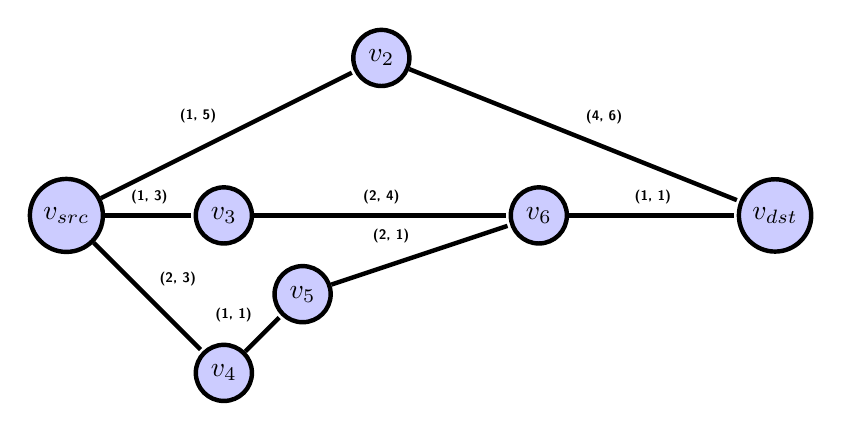
\begin{tikzpicture}[shorten >=1pt, auto, node distance=3cm, ultra thick,
   edge_style/.style={draw=black, ultra thick,font=\sffamily\tiny\bfseries}]
	  \node [circle,draw=black,fill=blue!20] (n1) at (1,2) {$v_{src}$};
	  \node [circle,draw=black,fill=blue!20] (n2) at (5,4)  {$v_2$};
	  \node [circle,draw=black,fill=blue!20] (n3) at (3,2)  {$v_3$};
	  \node [circle,draw=black,fill=blue!20] (n4) at (3,0)  {$v_4$};
	  \node [circle,draw=black,fill=blue!20] (n5) at (4,1)  {$v_5$};
	  \node [circle,draw=black,fill=blue!20] (n6) at (7,2)  {$v_6$};
	  \node [circle,draw=black,fill=blue!20] (n7) at (10,2) {$v_{dst}$};

	  \foreach \from/\to/\distance/\cost in {n1/n2/1/5, n1/n3/1/3, n1/n4/2/3, n3/n6/2/4, n5/n6/2/1, n4/n5/1/1, n6/n7/1/1, n2/n7/4/6}
	    \draw [edge_style] (\from) edge node{(\distance, \cost)} (\to);

	\end{tikzpicture}
	\caption{Ejemplo de conexion entre ciudades.} \label{fig:vida_real_1}
\end{figure}
Veamos 3 posibles caminos y analicemos cada uno:
\begin{itemize}
	\item $c_1$ = $<v_{src}, v_2, v_{dst}>$
		\begin{itemize}
			\item dist($c_1$) = 1 + 4 = 5
			\item costo($c_1$) = 5 + 6 = 11
		\end{itemize}
	\item $c_2$ = $<v_{src}, v_3, v_6, v_{dst}>$
		\begin{itemize}
			\item dist($c_2$) = 1 + 2 + 1 = 4
			\item costo($c_2$) = 3 + 4 + 1 = 8
		\end{itemize}
	\item $c_3$ = $<v_{src}, v_4, v_5, v_6, v_{dst}>$
		\begin{itemize}
			\item dist($c_3$) = 2 + 1 + 2 = 5
			\item costo($c_3$) = 3 + 1 + 1 = 5
		\end{itemize}
\end{itemize}
Supongamos que se dispone de K=9 para realizar el viaje, entonces veamos que el camino mas corto seria $c_1$ pero vemos que con esos costos se pasa de K=9, en particular el costo asociado a $c_1$ es 11. Entonces el mejor camino acotando el costo por 9 es $c_2$. Para instancias mas grandes, seguramente no ser\'a facil ver los caminos de esta forma o poder encontrar el \'optimo, ahi es cuando podemos modelar este problema utilizando CACM para lograr el objetivo.

\subsection{Camino mas conveniente segun relieve: Expedicion en la colina}
Otra posible aplicacion para este problema es la siguiente situacion: Se quiere ir de un punto A a otro B en un lugar geografico accidentado, donde existe una zona con un relieve complicado, llamemos C a esta zona, impidiendo cualquier camino directo entre A y B sin pasar por C. La zona accidentada, tiene varias estaciones de reabastecimiento para los viajantes. Procedamos a modelar con grafos la situacion: Sea G = (V, E) un grafo simple, los puntos A y B son dos nodos no adyacentes de G, ambos conectados a una componente conexa C(no necesariamente por una sola arista) (Figura \ref{fig:comp_conexa_ab_c}),luego, como C es conexa y A,B estan ambos conectados con C, existe al menos un camino entre A y B, que pasa por C. Dentro de C, los nodos denotan estaciones de reabastecimiento y si existe una arista entre dos nodos dentro de C, significa que se puede viajar entre dichas estaciones, mas formalmente:\\
Sean $v_1,v_2 \in V $ entonces $\exists $ $(v_1,v_2) \in E$ de peso $ (t, l) \in \mathbb{R_+}^2 \Leftrightarrow$ existe un sendero entre los puntos $v_{1}$ y $v_{2}$ con costo de l litros de nafta que toma t minutos en ser recorrido.
Cada una de las aristas ($v_i, v_j$), tanto entre A,B hacia C o mismas aristas contenidas en C, tienen asociadas dos funciones f,g definidas sobre el conjunto E de aristas del grafo G:
\begin{itemize}
	\item $f:E \rightarrow \mathbb{R}_+$: funcion asociada al tiempo de viaje en minutos entre $v_{i}$ y $v_{j}$.
	\item $g:E \rightarrow \mathbb{R}_+$: funcion asociada al costo de viajar entre $v_{i}$ y $v_{j}$, en cantidad de litros de nafta segun el terreno de dicho sendero.
\end{itemize}

\begin{figure}[H]
	\centering
	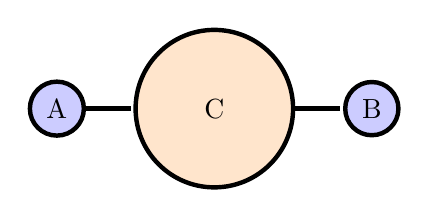
\begin{tikzpicture}[shorten >=1pt, auto, node distance=3cm, ultra thick,
   edge_style/.style={draw=black, ultra thick,font=\sffamily\tiny\bfseries}]
	  \node [circle,draw=black,fill=blue!20] (n1) at (1,2) {A};
	  \node [circle,draw=black,fill=orange!20, minimum size=2cm] (n2) at (3,2)  {C};
	  \node [circle,draw=black,fill=blue!20] (n3) at (5,2)  {B};

	  \foreach \from/\to in {n1/n2, n2/n3}
	    \draw (\from) -- (\to);

	\end{tikzpicture}
	\caption{Nodos A,B no adyacentes entre si, conectados a componente conexa C} \label{fig:comp_conexa_ab_c}
\end{figure}

El objetivo es llegar de A a B en la menor cantidad de tiempo, disponiendo de una cantidad fija $K\in \mathbb{R}_+$ de nafta para todo el viaje. Nuevamente este problema puede ser modelado utilizando CACM minimizando la funcion f tal que la funcion g quede acotada por la cantidad K de nafta.